\chapter{Regression Studies with Large Sample Windows}\label{app:large_window_regression}

The studies in this section were performed using the full large window samples, of size 51x51x25 in ECAL and 11x11x60 in HCAL.
%\footnote{/eos/project/d/dshep/LCD/DDHEP/*Escan\_*\_MERGED/}.
The samples consist of approximately 800,000 events for each particle type.  2/3 of the events were used for training and 1/3 of the events were used for testing.

The most important design choice found for the DNN/CNN networks is the size of the window used as input.  For both DNN and CNN, to achieve the best performance for energies above 150~GeV, a minimum $(x,y)$ size of 25x25 in the ECAL and 5x5 in the HCAL is needed.  For energies below 150~GeV, the optimal performance is observed for a window size of 51x51 in the ECAL and 11x11 in the HCAL.  This is presumably due to wider showers at low energy.  The impact of the choice of window size is shown for DNN in Figure~\ref{fig:reg_dnn_numcells}, with the results for CNN being similar.  Drawbacks to the larger window size, however, include larger files, more memory usage, and that training takes about 5 times longer per epoch.

\begin{figure}[htbp]
\centering
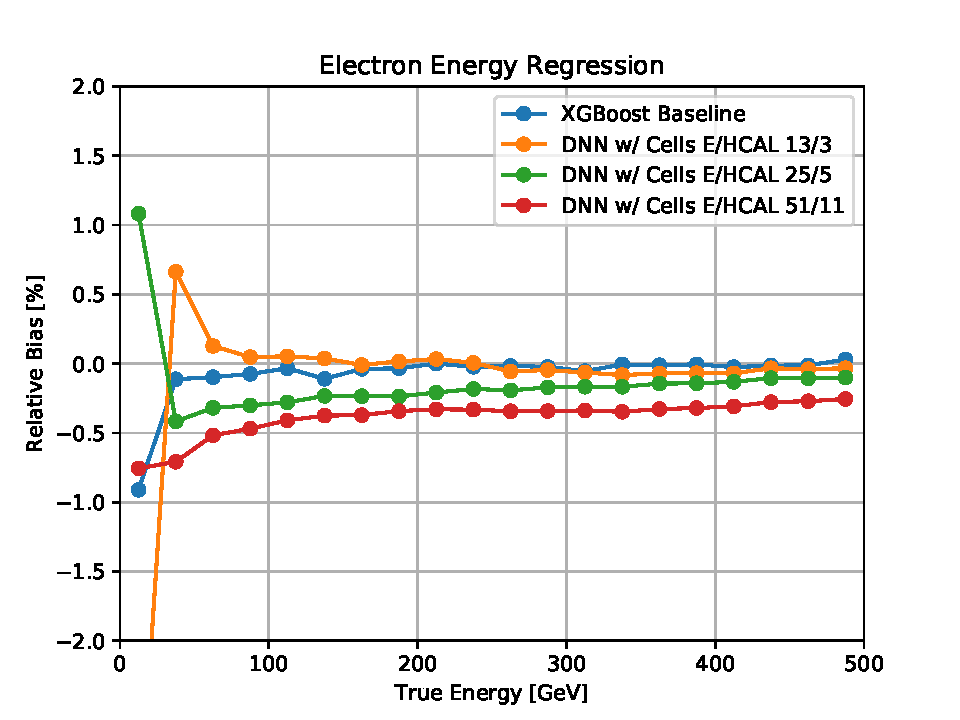
\includegraphics[width=0.38\textwidth]{Images/Calo/bias_vs_E_EleFixed_nn_numcells_zoom.pdf}
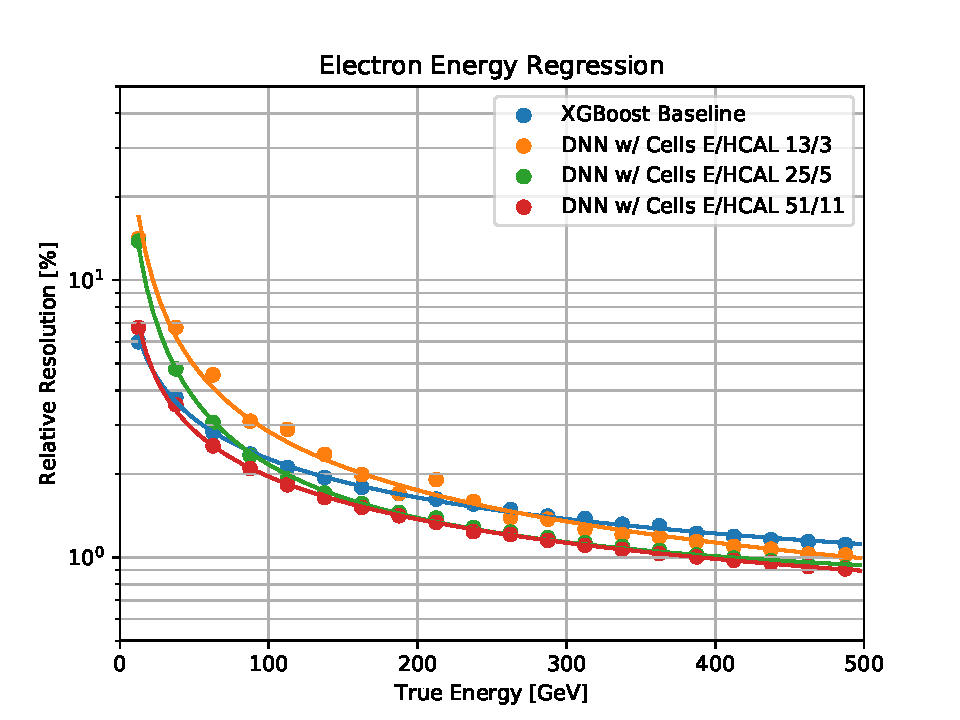
\includegraphics[width=0.38\textwidth]{Images/Calo/res_vs_E_EleFixed_nn_numcells_fits.pdf}
\caption{Bias (top) and resolution (bottom) as a function of true energy for DNN energy predictions for electrons, with varying input window sizes.
}
\label{fig:reg_dnn_numcells}
\end{figure}

Showers for \chpi\ were observed to be wider than the other particle types, especially at low energies, and so we compare the effect of the calorimeter window size choice for \chpi\ in Figure~\ref{fig:reg_nn_numcells_chpi_large_window}.  The wider window of 51x51 in $(x,y)$ in the ECAL and 11x11 in the HCAL gives better performance, especially at the lowest energies where the resolution is improved by a factor of about 2 over the smaller window size (25x25 ECAL, 5x5 HCAL).

\begin{figure}[htbp]
\centering
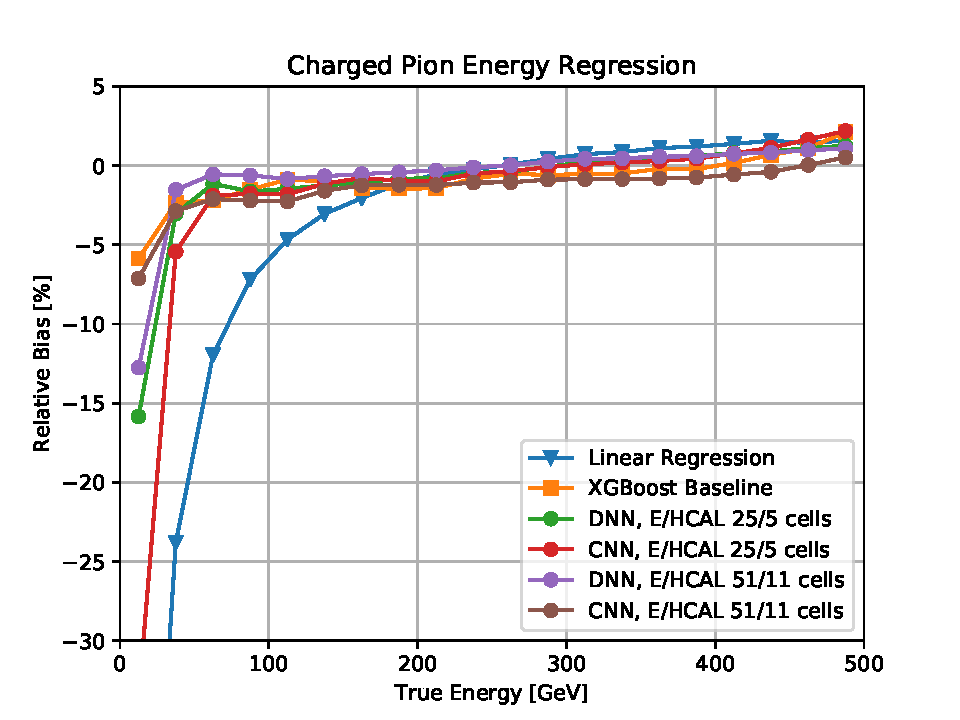
\includegraphics[width=0.38\textwidth]{Images/Calo/bias_vs_E_ChPiFixed_Cut30_nn_numcells.pdf}
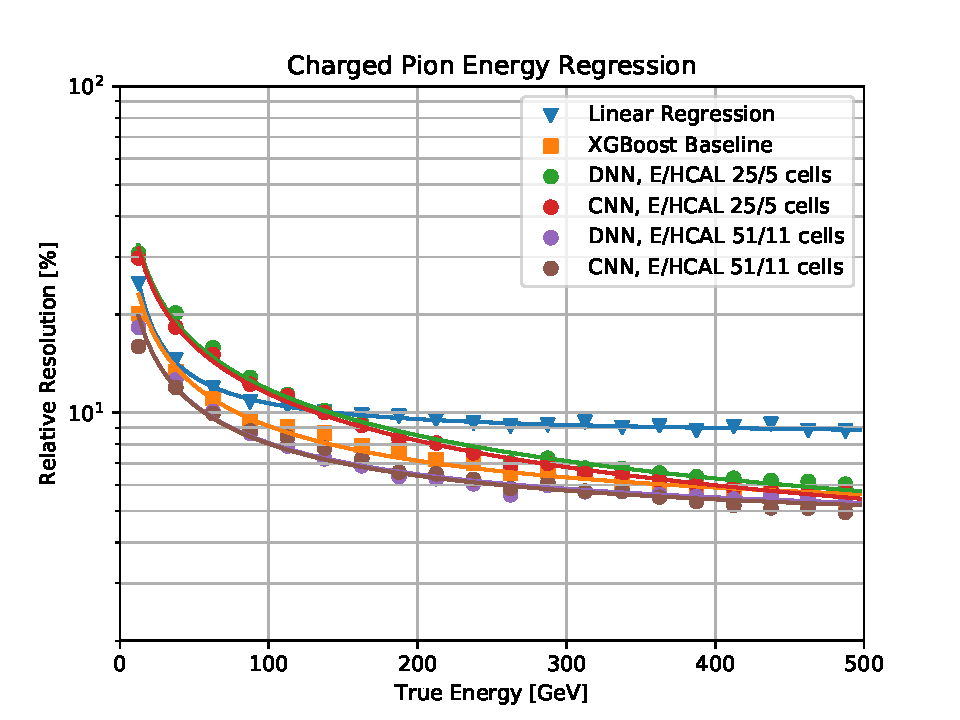
\includegraphics[width=0.38\textwidth]{Images/Calo/res_vs_E_ChPiFixed_Cut30_nn_numcells_fits.pdf}
\caption{Bias (top) and resolution (bottom) as a function of true energy for energy predictions for \chpi, comparing calorimeter window sizes for the CNN and DNN models.
}
\label{fig:reg_nn_numcells_chpi_large_window}
\end{figure}

\chapter{Skip Connections for Regression}\label{app:skip_connections}

A design choice that improved convergence time, and improved performance for the CNN, is including ``skip connections'' for the total ECAL and HCAL energies in the network.  In addition to the individual cell energy values, the total ECAL and HCAL energy values are given as inputs to both the first dense layer and to the last output layer.  The weights for these energy values are initialized to 1, as linear regression with coefficients near 1 is observed to reasonably reproduce the true energy values.  The impact of adding skip connections on performance using a CNN architecture for a fixed number of 5 training epochs is shown in Figure~\ref{fig:reg_cnn_skip}.

\begin{figure}[htbp]
\centering
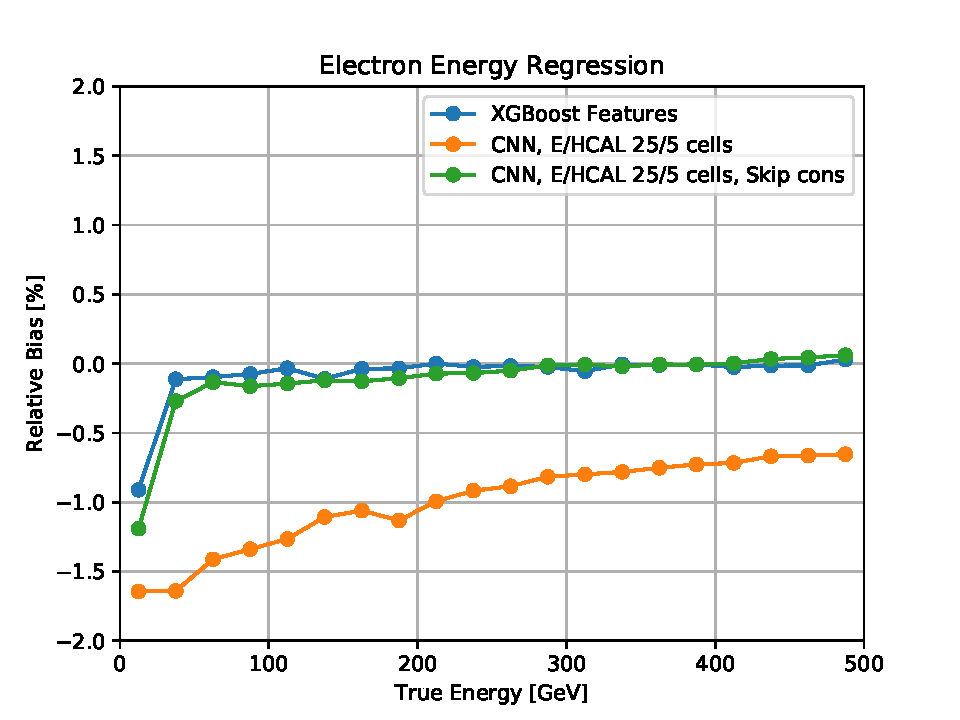
\includegraphics[width=0.38\textwidth]{Images/Calo/bias_vs_E_EleFixed_cnn_skip_zoom.pdf}
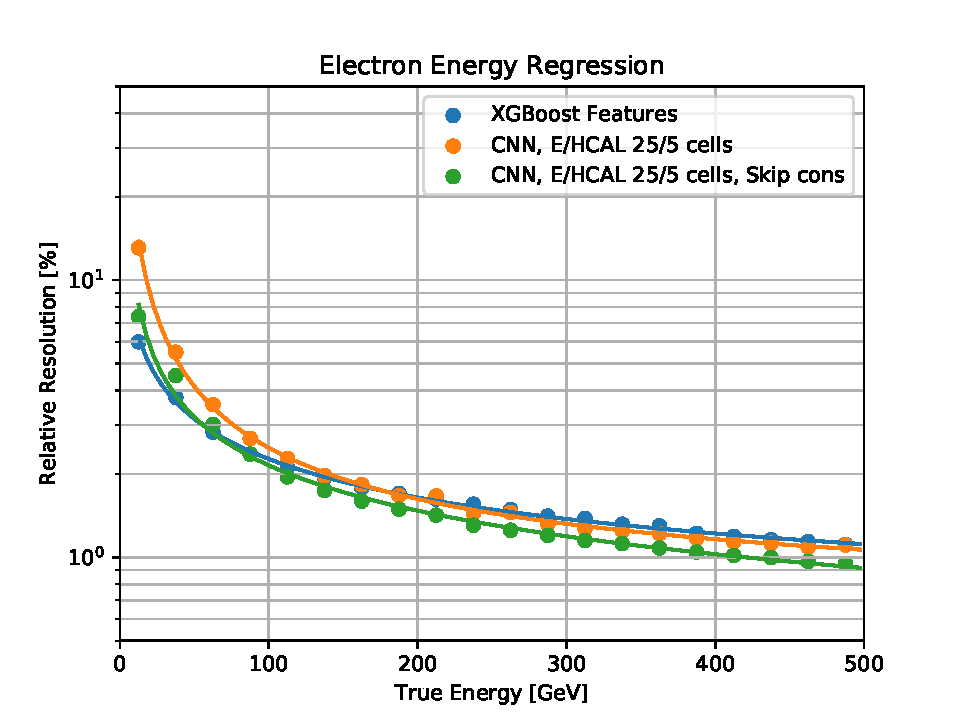
\includegraphics[width=0.38\textwidth]{Images/Calo/res_vs_E_EleFixed_cnn_skip_fits.pdf}
\caption{Bias (top) and resolution (bottom) as a function of true energy for CNN energy predictions for electrons, with or without skip connections in the architecture.
}
\label{fig:reg_cnn_skip}
\end{figure}